%!TEX root = ./template-skripsi.tex
%-------------------------------------------------------------------------------
% 								BAB I
% 							LATAR BELAKANG
%-------------------------------------------------------------------------------

\chapter{PENDAHULUAN}

\section{Latar Belakang Masalah}

Indonesia memiliki dua sumber perikanan: tangkap laut dan budidaya ikan air tawar. Tidak seperti memancing di laut, budidaya ikan air tawar membutuhkan lebih banyak modal untuk melakukan hal-hal seperti infrastruktur lahan, kolam/renang dan juga pemberian makan. BelumApalagi budidaya ikan  tidak mudah dan membutuhkan keahlian khusus. NamunIni tidak berarti bahwa ikan yang ditangkap memiliki kendali penuh atas pasar hasil tangkapandengan mempertimbangkan beberapa pertimbangan yaitu rasa ikan air tawar dan ikan air asin berbeda,Ikan air tawar  dapat dipasarkan dalam kondisi hidup, biaya dan waktupengiriman tidak cukup untuk mencapai daerah pegunungan untuk mengirimmenangkap ikan. Dengan modal yang besar tentunya  juga membutuhkandengan nilai ekonomi potensial.

\begin{figure}[H]
	\centering
	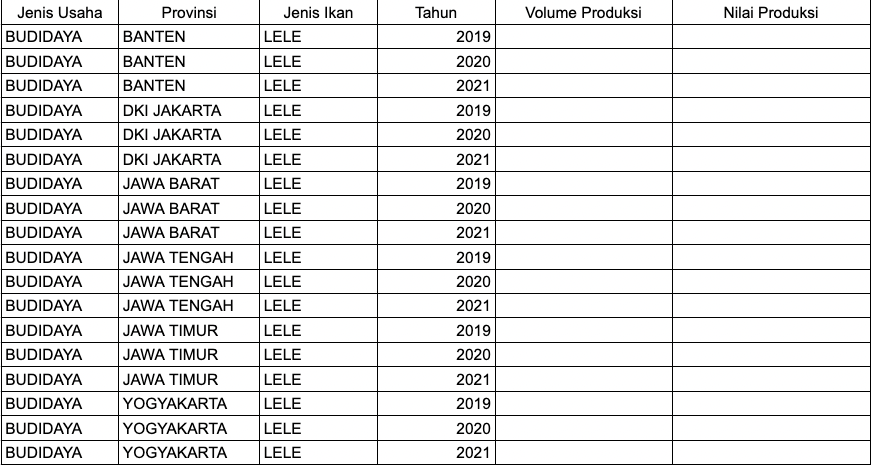
\includegraphics[keepaspectratio, width=12cm]{gambar/budidaya-ikan-lele-jawa.png}
	\caption{\emph{Produksi Ikan Lele Di Pulau Jawa} \citep{kkpdatajawa}}
	\label{gambar:budidaya-ikan-lele-jawa}
\end{figure}

\section{Rumusan Masalah}
Dari uraian latar belakang di atas, perumusan masalah pada penelitian ini ialah “Bagaimana perancangan aplikasi yang mendukung \emph{multi user} dan inventarisasi yang menjadi pendukung dalam menjalankan budidaya perikanan modern?”

\section{Pembatasan Masalah}
Pembatasan masalah pada penelitian ini antara lain:
\begin{enumerate}
	\item Aplikasi dikembangkan untuk banyak user.
	\item Pengembangan aplikasi menggunakan \emph{Framework} Flutter.
	\item Pengembangan \emph{web service} menggunakan \emph{Framework} Flask.
\end{enumerate}

\section{Tujuan Penelitian}
	Penelitian ini dilakukan dengan tujuan untuk membuat aplikasi budidaya ikan modern dengan penerapan \emph{multi user} dan inventarisasi berbasis \emph{multi platform}.

\section{Manfaat Penelitian}
\begin{enumerate}
	\item Bagi penulis
		
	Meningkatkan pengetahuan tentang teknologi budidaya perikanan modern, menambah pengalaman dalam mengembangkan aplikasi, memperoleh gelar sarjana di bidang Ilmu Komputer, serta menjadi media untuk penulis dalam mengaplikasikan ilmu yang didapat dari kampus.
		
	\item Bagi Universitas Negeri Jakarta
	 	
	Menjadi pedoman untuk penelitian di masa depan, dan dapat memberikan panduan bagi mahasiswa program studi Ilmu Komputer tentang rancang bangun aplikasi teknologi budidaya perikanan modern.
	
	\item Bagi masyarakat
	 	
	Membantu masyarakat yang ingin dan sedang menggeluti bidang budidaya perikanan dalam proses pendataan ikan dan pengelolaan lingkungan dalam budidaya itu sendiri.
	 			
\end{enumerate}


% Baris ini digunakan untuk membantu dalam melakukan sitasi
% Karena diapit dengan comment, maka baris ini akan diabaikan
% oleh compiler LaTeX.
\begin{comment}
\bibliography{daftar-pustaka}
\end{comment}
